\documentclass[11pt]{article}
\bibliographystyle{IEEEtran}
\usepackage[bookmarks=false]{hyperref}
% Listing (fold)
\usepackage{listings} 
\usepackage{textcomp} %for upquotes 
                           
\lstset{
	tabsize=4,
	mathescape=true, 
	escapechar=§,
	upquote=true,
	basicstyle=\ttfamily,
} %(end)

% Pictures (fold)
\usepackage[pdftex]{graphicx}
\usepackage{subfigure}
\usepackage{wrapfig} % (end)

% Geometry (fold)
\usepackage[pdftex]{graphicx}
\usepackage{geometry}
\geometry{bottom=2.4cm, top = 2.4cm}
\renewcommand{\topfraction}{0.97}	% max fraction of floats at top
\renewcommand{\bottomfraction}{0.97}	% max fraction of floats at bottom
\renewcommand{\textfraction}{0.01}

% Very small margins
% \geometry{left=1.5cm, right=1.5cm, bottom=1.9cm, top = 1.9cm}
% (end)

% Maths (fold)
\usepackage{amsmath}
\usepackage{amssymb}
\usepackage{amsthm}
\usepackage{ wasysym } %Bowtie for na join (end)             

% Other Packages (fold)
% Makes small lists
\usepackage{enumitem}
\usepackage[utf8]{inputenc}
%(end)

% Not on Packages/Settings (fold)
%small sections
 % \usepackage[small,compact]{titlesec}
% Small text nicer
 % \usepackage{microtype}

% \usepackage{alltt}
% \renewcommand{\ttdefault}{txtt}

% \usepackage[bookmarks=true]{hyperref}
% \setcounter{secnumdepth}{5}
% \setcounter{tocdepth}{5}

% (end)

% shortcuts (fold)
\def\studentID{080008164}
\def\fullName{Bilal Hussain}
\newcommand{\picwidth}{6.3in}

\def\*{\ensuremath{\times}}
\def\<={\ensuremath{\leqslant}}
\def\>={\ensuremath{\geqslant}}
\def\={\ensuremath{\neq}}
\def\~{\ensuremath{\approx}}

\def\s{\textsuperscript{* }}
\def\ts{\textsuperscript}
\def\-{\subscript}
\def\_{\textunderscore}
\def\set#1{\{ #1 \}}
\def\t#1{\text{#1}}

\def\abs#1{\mathopen| #1 \mathclose|}
\def\Integer{\mathsf{Z\hspace{-0.4em}Z}}
\def\Natural{\mathrm{I\!N}}
\def\Real{\mathrm{I\!R}}
%(end)

%p code	(fold)
\def\And{\ensuremath{\textbf{ and }}}
\def\Not{\ensuremath{\textbf{ not }}}
\def\Xor{\ensuremath{\textbf{ xor }}}
\def\Or{\ensuremath{\textbf{ or }}}

\def\If{\ensuremath{\textbf{if }}}	
\def\For{\ensuremath{\textbf{for }}}	
\def\While{\ensuremath{\textbf{while }}}
\def\Else{\ensuremath{\textbf{else }}}
\def\Do{\ensuremath{\textbf{ do}}}
\def\To{\ensuremath{\textbf{ to }}}
\def\Then{\ensuremath{\textbf{ then}}}
\def\Until{\ensuremath{\textbf{ until }}}
\def\End{\ensuremath{\textbf{end}}}
\def\Downto{\ensuremath{\textbf{ downto }}}

\def\Swap{\ensuremath{\textbf{swap }}}
%(end)

% Metadata
\newcommand{\theTitle}{}
\title{\theTitle}
\author{\studentID}

% Headers footers (fold)             

%	default Headers
% \pagestyle{headings}

\usepackage{fancyhdr} 
\pagestyle{fancy}
\fancyhf{} % removes all headers
\fancyhead[CEO]{\hspace{10pt} \theAuthor \hspace{5pt}-- \theTitle}
\fancyfoot[CEO]{\thepage} % (end)      
\renewcommand{\theTitle}{A Tactical RPG Engine}
\renewcommand{\theAuthor}{\fullName}

\begin{document} 
\maketitle


\section{Introduction} 
\label{introduction}


A RPG (Role Playing Game) is game where player assumes the role of on the character. A RPG is usually story driven and the character usually has quest to complete. In the course of the game the player will go to different environments such as town and dungeons. In they these environments the player will have to battle opponents in battles. Combat in RPGs is normally a simple turn based system where player and the opponents take turns attacks each other using various skills. 

A Tactical RPG is sub-genre of an RPG that focuses on the combat side of the genre. A Tactical RPG is series of \texttt{battles}, which take place in various environments intertwined with an over-aching story.

Each \texttt{battle} is grid based (like chess) where each player has a number of units(pieces). 
\begin{figure}
	[htbp] \centering 
	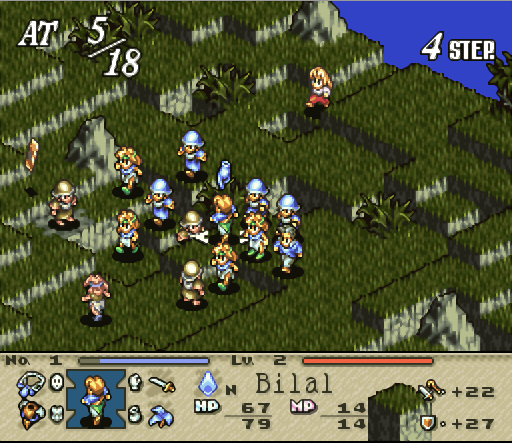
\includegraphics[height=3in]{figures/TRPG.png} \caption{\textbf{Tactics Ogre}\cite{to} a classic Tactical RPG } \label{fig:figures_TRPG} 
\end{figure}
The players taken turns to moves their units. Each unit has attributes associated with it such as strength, and hit points that affect all the actions in the game. Like chess there are different kinds of units which affects how the unit moves and what action they can perform. A unit can attack other player's units, the goal of the battle is usually to defeat all the opponents units.

The aim of this project is to create a engine which will take resources such as graphics, sound and rules of the game to create a runnable Tactical RPG.

\section{Objectives}

\subsection{Primary}
 \label{primary}
\begin{itemize}
\item To develop an engine that takes:
\begin{itemize}

 \item The definition of character attributes and a combat system.
	\item The definition of a world broken up into the smaller environments.
	\begin{itemize}
		\item The rules of the game.
		\item The kinds of enemies.
	\end{itemize}
	
	\item The definition of simple story as a wrapper for the whole game, from the start to the conclusion of the game
	\begin{itemize}
		\item Which is told between the movement between different environments.
	\end{itemize}
	                        
	\item The set of selected character attributes.
	
\end{itemize}
and create a playable tactic RPG.

\item To include in the engine support for the following:
\begin{itemize}
	\item \texttt{units} with a fixed set of associated attributes such as:
	\begin{itemize}
		\item Hit-points (which represent the health of the unit).
		\item Strength.
		\item Defence.
		\item Move (The number of tiles the unit can move each turn).
	\end{itemize}
	
	\item \texttt{battles} which take place on grid and include:
	\begin{itemize}
		\item A set number of \texttt{units} for each player.
		\item A Winning \texttt{condition} such as defeat all of the other players units.
		\item Battles are \texttt{turn based} meaning that each player moves all their units (once) before the next player turn.   
		\item A combat system.
	\end{itemize}
	
	\item A combat system that includes
		\begin{itemize}
			\item \texttt{combat} between adjacent units.
			\begin{itemize}
				\item When the unit hit-points are reduced to zero they are \texttt{defeated} and are removed from the map
			\item A set of rules that govern the combat.
			\end{itemize}
			
		\end{itemize}
	
	\item A predefined set of behaviours for how the non-player characters should behave.
	\begin{itemize}
		\item Including pathfinding.
	\end{itemize}
	
	\item A simple graphical representation of of the game.
	\begin{itemize}
		\item Which is show the grid with all the units.
		
		\item Allow the user to move their units and see the opponents moves.
		
		\item Allows the user to attack the opponents units.
	\end{itemize}
\end{itemize}
\end{itemize}

\subsection{Secondary} 
\label{secondary}
\begin{itemize}
	\item Tile \texttt{height}, where units can only move to tiles of a smilier height.
	
	\item Tiles that are not passable such as sea, lava, etc.
	
	\item Tiles have different movement costs associated with them.
	
	\item Isometric graphics view of the game.
	
	\item Long distance weapons\slash magic for player and AI.
	
	\item Direction and height of the character's tile affects attack.
	
	\item Sound effects.
	
	\item Music.
	
	\item Saving and loading games.
	
	\item Allow the user to specify some of behaviour of non-player characters
	\begin{itemize}
		\item Such as always attack a certain kind of unit or always attack the unit with the most Hit Points.
	\end{itemize}
	
	\item A graphical view to allow user specify the input to the engine.
\end{itemize}

\subsection{Tertiary} 
\label{tertiary}
\begin{itemize}
	\item Custom events
	\begin{itemize}
		\item Attached to units or titles, could be used for:
		\begin{itemize}
			\item Making the player win if some enemies unit has less then 50\% Hit Points.
			
			\item Damaging a character if step on a specified.
			
			\item Showing some part of the story when a player's character reach a specified tile.
		\end{itemize}
	\end{itemize}
	
	\item A graphical editor for making custom maps and events.
	
	\item Healing item\slash skills.
	
	\item Animations for units, combat and movement.
\end{itemize}

\subsection{Ethical Considerations} 
\label{ethicalconsiderations}
\begin{itemize}
	%\item Form by 28th October.
	
	\item Collection of data from questionnaire.
	\begin{itemize}
		\item Just result of questionnaire, no personal data.
	\end{itemize}
	
	\item Asking users to create a game.
	
	\item Asking users to play the created game.
\end{itemize}

\subsection{Resources} 
\label{resources}
\begin{itemize}
	\item None.
\end{itemize}

\bibliography{Citations}
\end{document}
